% Generated by TikzMakie.jl. Requires \usepackage{tikz} (and graphicx if images are used).
\begin{tikzpicture}[x=0.75pt, y=0.75pt, mknode/.style={inner sep=0pt, outer sep=0pt, execute at begin node={\vphantom{(}}, font=\fontsize{10.5}{12.6}\selectfont}, mkimg/.style={inner sep=0pt, outer sep=0pt}]
\path[use as bounding box] (0,0) rectangle (560,420);
\path[fill=white] (101,56) -- (430,56) -- (430,386) -- (101,386) -- cycle;
\draw[draw=black, line width=0.75pt, draw opacity=0.12]
  (158.57,56) -- (158.57,386)
  (265.5,56) -- (265.5,386)
  (372.42,56) -- (372.42,386);
\draw[draw=black, line width=0.75pt, draw opacity=0.12]
  (101,113.75) -- (430,113.75)
  (101,221) -- (430,221)
  (101,328.25) -- (430,328.25);
\node[mknode, anchor=north] at (265.5,28.69) {$x$};
\node[mknode, anchor=north] at (158.57,48) {$-2$};
\node[mknode, anchor=north] at (265.5,48) {$0$};
\node[mknode, anchor=north] at (372.42,48) {$2$};
\node[mknode, anchor=south, rotate=90] at (70.04,221) {$y$};
\node[mknode, anchor=east] at (91,113.75) {$-2$};
\node[mknode, anchor=east] at (91,221) {$0$};
\node[mknode, anchor=east] at (91,328.25) {$2$};
\node[mknode, anchor=south, font=\fontsize{10.5}{12.6}\selectfont\bfseries] at (265.5,390) {$z = \sin x \cos y + 0.3x$};
\begin{scope}
\clip (101,56) rectangle (430,386);
\node[mkimg, anchor=south west] at (101,56) {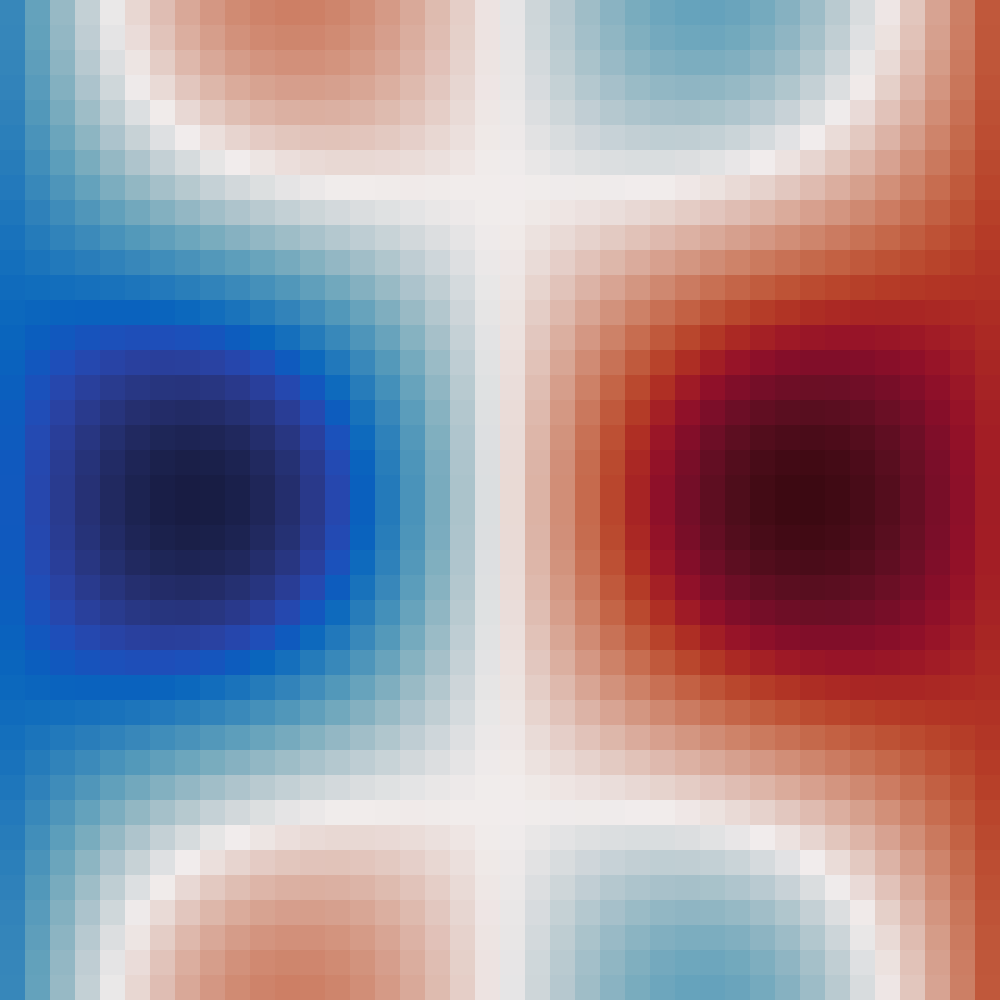
\includegraphics[width=246.75pt, height=247.5pt]{06_heatmap-1.png}};
\end{scope}
\node[mkimg, anchor=south west] at (489,56) {
\includegraphics[width=9pt, height=247.5pt, interpolate=true]{06_heatmap-2.png}};
\draw[draw=black, line width=0.75pt, miter limit=2]
  (501,56) -- (501,386) -- (489,386) -- (489,56) -- (501,56);
\node[mknode, anchor=north, rotate=90] at (530.96,221) {$z$};
\node[mknode, anchor=west] at (510,111.93) {$-1$};
\node[mknode, anchor=west] at (510,221) {$0$};
\node[mknode, anchor=west] at (510,330.07) {$1$};
\draw[draw=black, line width=0.75pt]
  (158.57,55.5) -- (158.57,50.5)
  (265.5,55.5) -- (265.5,50.5)
  (372.42,55.5) -- (372.42,50.5);
\draw[draw=black, line width=0.75pt]
  (100.5,113.75) -- (95.5,113.75)
  (100.5,221) -- (95.5,221)
  (100.5,328.25) -- (95.5,328.25);
\draw[draw=black, line width=0.75pt]
  (501.5,111.93) -- (506.5,111.93)
  (501.5,221) -- (506.5,221)
  (501.5,330.07) -- (506.5,330.07);
\draw[draw=black, line width=0.75pt]
  (100.5,56) -- (430.5,56);
\draw[draw=black, line width=0.75pt]
  (101,55.5) -- (101,386.5);
\draw[draw=black, line width=0.75pt]
  (100.5,386) -- (430.5,386);
\draw[draw=black, line width=0.75pt]
  (430,55.5) -- (430,386.5);
\end{tikzpicture}
